\documentclass[doc,a4paper,12pt]{apa6}
\usepackage[a4paper]{geometry} 
\usepackage[utf8]{inputenc}
\usepackage[T1]{fontenc}
\usepackage[ngerman]{babel}
\usepackage{amsmath}
\usepackage[doublespacing]{setspace}
\usepackage{paralist}
\usepackage{graphicx}
\usepackage{epstopdf}
\usepackage{wrapfig}
\usepackage{float}
\usepackage{csquotes}
\usepackage[hidelinks]{hyperref}
\usepackage[backend=biber,style=apa]{biblatex}
\usepackage[titles]{tocloft}

\DeclareLanguageMapping{ngerman}{ngerman-apa}
\DefineBibliographyStrings{ngerman}{andothers={et\ al\adddot}}

\bibliography{references}
 
\title{Explizite Detektion von Abweichungen in komplexen Regeln bei auditiven Stimuli}
\shorttitle{Explizite Komplexe Regelerkennung}
\author{Carlo Michaelis}
%\date{23. August 2013}
%\affiliation{geb. am 29.09.1989 in Dieburg\\ Institut für Psychologie, Universität Leipzig\\ \ }
%\note{\textbf{Gutachter}:\\ (1) Frau Prof. Dr. Alexandra Bendixen\\ (2) Herr Prof. Dr. Erich Schröger\\ \ \\ Dieses Dokument ist unter folgender Lizenz veröffentlicht:\\ Creative Commons (CC BY 3.0)}

\renewcommand{\cftfigpresnum}{Abb. }
\settowidth{\cftfignumwidth}{Abb. 10\quad}

\geometry{a4paper, bottom=1.5in}
\setlength{\skip\footins}{1.5em}
\setlength{\footnotesep}{1.5em}
\setlength{\textfloatsep}{2em}
\raggedbottom
\begin{document}

%\maketitle

\thispagestyle{empty}

\begin{spacing}{1.1}
\begin{center}

\Large Universität Leipzig

\setlength{\parskip}{0.8em}
\normalsize Fakultät für Biowissenschaften, Pharmazie und Psychologie

\setlength{\parskip}{0.4em}
\normalsize Institut für Psychologie

\setlength{\parskip}{6em}
\LARGE \textbf{Explizite Detektion von Abweichungen in komplexen Regeln bei auditiven Stimuli}

\setlength{\parskip}{1.8em}
\normalsize Abschlussarbeit zur Erlangung des akademischen Grades\\ Bachelor of Science (B.Sc.)

\setlength{\parskip}{1.2em}
\normalsize vorgelegt von

\setlength{\parskip}{1.8em}
\Large \textbf{Carlo Michaelis}

\setlength{\parskip}{0.5em}
\normalsize geb. am 29.09.1989 in Dieburg

\setlength{\parskip}{3em}

Erstgutachterin: Frau Prof. Dr. Alexandra Bendixen

\setlength{\parskip}{0.3em}
Zweitgutachter: Herr Prof. Dr. Erich Schröger

\vfill

Dieses Dokument ist unter folgender Lizenz veröffentlicht:\\ \href{http://creativecommons.org/licenses/by/3.0/de/}{Creative Commons (CC BY 3.0 DE)}

\end{center}
\end{spacing}
\newpage

\section*{Selbstständigkeitserklärung}

Ich versichere hiermit, dass ich die vorliegende Arbeit selbständig verfasst und keine
anderen als die im Literaturverzeichnis angegebenen Quellen benutzt habe.\\
Alle Stellen, die wörtlich oder sinngemäß aus veröffentlichten oder noch nicht veröffentlichten
Quellen entnommen sind, sind als solche kenntlich gemacht.\\
Die Zeichnungen oder Abbildungen in dieser Arbeit sind von mir selbst erstellt worden oder
mit einem entsprechenden Quellennachweis versehen.\\
Diese Arbeit ist in gleicher oder ähnlicher Form noch bei keiner anderen Prüfungsbehörde
eingereicht worden.

\vspace{3em}
\noindent Leipzig, den 12.11.2013\\ Carlo Michaelis

\newpage

\section*{Zusammenfassung}

Die vorliegende Arbeit thematisiert die Verarbeitung komplexer Regeln bei auditiven Stimuli. Untersucht wurde auf welcher Ebene solche komplexen Regeln verarbeitet werden.

Vorige Studien zeigten bereits, dass das Gehirn die Fähigkeit besitzt solche Regeln präattentiv auf sensorischer Ebene zu erkennen. Insbesondere hat das Gehirn die Fähigkeit Abweichungen solcher Regeln zu erkennen. Die sensorische Erkennungsleistung wurde mittels der Mismatch Negativity (MMN) nachgewiesen.

Die vorigen Experimente wurden in dieser Untersuchung auf einen expliziten Lernprozess erweitert und es wurde geprüft, ob die Erkennung von Abweichungen solcher Regeln auch explizit erlernbar ist. Dafür bekamen die Versuchspersonen die Regeln ausführlich erläutert und hatten die Möglichkeit diese Regeln langsam zu üben. Erhoben wurden in diesem Experiment ausschließlich behaviorale Daten in Form von Sensitivität und Reaktionszeit. Im Ergebnis zeigte sich zunächst, dass die Erkennungsleistung der Regelabweichungen trotz der Übung nicht zunahm und somit kein explizites oder implizites Lernen vorlag. Komplexe auditive Regeln scheinen nur auf sensorischer Ebene verarbeitet zu werden.

Weitere Auswertungen der Daten ergaben eine geringe Evidenz für leichte Lerneffekte. Sollte explizites Lernen solcher Regeln möglich sein, dann vermutlich nur unter sehr hohem zeitlichem und konzentrativem Aufwand. Effekte von Musikalität und unterschiedlicher angewendeter Strategien der Versuchspersonen lagen nicht vor.

Es bleibt festzuhalten, dass der Mensch über ein hoch effektives Erkennungssystem verfügt, welches auch ohne Verwendung von Aufmerksamkeitsressourcen komplexe Regeln schnell erkennen und Fehler darin zuverlässig detektieren kann.

\newpage

\setcounter{tocdepth}{2}
\tableofcontents
\newpage

\listoffigures
\newpage

\section{Einleitung}

Viele Fragen sind bis heute ungeklärt und werden es wohl auch weiterhin bleiben. Trotzdem scheint es, als gäbe es – vor allem bei der Erklärung unserer physikalischen Umgebung – schon einige befriedigende Antworten, die es uns nicht nur ermöglichen, unser Leben gesund und sicher zu gestalten, sondern auch unseren Hunger nach Verständnis großteils decken. Auch im Bereich psychischer Prozesse gibt es bereits verschiedene Einzelerkenntnisse, eine umfassende Theorie über die psychischen Funktionsweisen komplexerer Organismen steht jedoch aus. Vor allem das Zusammenspiel, also die Schnittstelle zwischen der Psyche und dem Körper, die Frage nach Determiniertheit und Selbstbestimmung, nach automatischer und willentlicher Verarbeitung sind bei weitem noch nicht vollständig geklärt.\\
Dabei erfüllt das Verständnis darüber nicht nur den Zweck, Wissen über Lebewesen zu akkumulieren oder einige neugierige Personen zu befriedigen, vielmehr prägt die Erkenntnis über die Funktionsweise unsere Gesellschaft: Sie entscheidet u.\,a. über Gesetze, Konventionen und Kultur.\\
So sehr und so selbstverständlich wir Menschen uns auch immer wieder einen freien Willen unterstellen und damit die Fähigkeit, durch den Geist gezielt und indeterminiert unsere Welt verändern zu können; ohne unwillkürlich automatisch ablaufende Verhaltensweisen wäre ein Leben auf der Erde wohl unmöglich. In vielen Situationen müssen innerhalb kürzester Zeit bestehende Reize erfasst, zukünftige Ereignisse simuliert und schließlich vorhergesagt werden.

Ein gutes Beispiel für die hohe Leistungsfähigkeit der automatisch ablaufenden Systeme des Menschen ist seine Sprache. Deutlich wird dies schon allein durch das Segmentationsproblem des Sprachverstehens. Mit physikalischen Mitteln aufgezeichnete Frequenzen von Schallwellen zeigen Muster, die bei visueller Betrachtung kaum korrekt in Worte getrennt werden können. Eine Pause oder eine Frequenzschwankung sagt nur selten tatsächlich auch den Beginn eines neuen Wortes vorher. Zur Segmentation der Worte werden bei weitem nicht nur die physikalischen Signale, sondern zusätzlich viele verschiedene Hinweisreize benötigt \parencites[u.\,a.][]{brent1996distributional}{saffran1996word}. Wichtig sind vor allem Lautfolgen, die in verschiedenen Sprachen nur mit einer bestimmten Wahrscheinlichkeit oder sogar gar nicht vorkommen. Die Folge von `x' und `s' würde in der Deutschen Sprache nicht erwartet werden und liefert dem auditiven System keine semantische Information. Das System würde in diesem Fall eher von zwei Wörtern ausgehen. Eines, das auf `x' endet, und eines, das mit `s' beginnt (z.B. `Max sieht'). Dabei muss die Segmentation nicht nur anhand einer großen Menge an Informationen, sondern auch innerhalb kürzester Zeit erfolgen, die ohne eine automatisierte Verarbeitung kaum möglich wäre. \textcite{sanders2002segmenting} fanden Hinweise, dass die Segmentation automatisch abläuft, sofern die zu segmentierende Sprache der Muttersprache entspricht oder die Sprache gut gelernt ist.

Beim Sprechen wiederum ist unter anderem das so genannte Speech Monitoring \parencites{levelt1983monitoring}{postma2000detection} von hoher Bedeutung. Das bezeichnet die Fähigkeit, die inhaltliche Qualität des Gesprochenen noch während des Sprechens reflektieren zu können. Das wiederum bedeutet, dass beim Sprechen mindestens zwei Prozesse gleichzeitig stattfinden: Sprachproduktion und Monitoring. Das legt nahe, dass hier ein hoher Grad an automatischer Verarbeitung im Spiel ist. In einer Studie von \textcite{goldman1958speech} konnte gezeigt werden, dass u.\,a. immer dann größere Sprechpausen entstehen, wenn kommende Wörter schwerer vorhersagbar sind. Das lässt vermuten, dass an diesen Stellen eine automatische Verarbeitung nicht mehr vollständig möglich ist und eine bewusste Verarbeitung zumindest teilweise einsetzt.

Bezüglich der auditiven Komponente sei vor allem auch die Musik hervorgehoben. Gerade in der Musik spiegelt sich die Tendenz des Menschen zu erfolgreichen automatischen Vorhersagen wider. \textcite{drake2001quest} prüften 5~universelle, d.h. nicht-kulturabhängige Paradigmen, wie sich Menschen zu Musik verhalten. In Paradigma~3 beschrieben sie, dass sich Menschen, die im Takt der Musik bleiben sollten, in mehr als 90\% der Zeit erfolgreich mit Musik synchronisieren können. D.\,h. Vorhersagen können erfolgreich getroffen und Handlungen an den Vorhersagen ausgerichtet werden; ein Verhalten, das auch bei unmusikalischen Menschen auftritt und damit auch hier einen Hinweis für ein automatisches Verhalten liefert. Man könnte mutmaßen, dass in der Vorhersagbarkeit, die anscheinend mehr passiv mit dem Menschen geschieht, als dass diese aktiv hervorgerufen wird, der Reiz der Musik liegt und auch ein Harmonieempfinden damit zusammenhängt.

Die Bedeutung der Vorhersagbarkeit und vor allem der diesbezüglich wirkenden automatischen Verarbeitung lassen sich an den vorigen Beispielen erkennen. In der folgenden Beschreibung des Experiments soll es um die Vorhersagbarkeit von komplexen Regeln in auditiven Stimuli gehen. Konkret wurde untersucht, inwiefern komplexe Regeln von Tonabfolgen (wie sie etwa auch in der Sprache vorkommen) erkannt und insbesondere vorhergesagt bzw. Abweichungen erkannt werden können. Im Folgenden soll zunächst der Forschungsstand bezüglich der auditiven Regelerkennung und der Vorhersagefähigkeit erläutert werden. Anschließend folgt eine kurze Einführung in die Lerntheorien, die speziell für dieses Experiment von Bedeutung sein wird. Und zuletzt soll in der Diskussion und der folgenden Post-Hoc-Analyse versucht werden, die genannten Beispiele einzuordnen.

\subsection{Mismatch Negativity (MMN) und das Oddball Paradigma}

Die Mismatch Negativity (MMN) ist ein ereigniskorreliertes Potential (EKP). Dabei handelt es sich um elektrische Potentiale des Gehirns, welche zu einem bestimmten Zeitpunkt (Ereignis) eintreten und mit diesem zusammenhängen und daher als ereigniskorreliert betrachtet werden können. Die Messung dieser Signale erfolgt per Elektroenzephalogramm (EEG), das elektrische Potentiale des Gehirns erfassen kann. Um die Signale, die durch das Ereignis ausgelöst werden, letztlich vom Rauschen anderer Gehirnpotentiale trennen zu können, werden die Potentiale über mehrere Messungen gemittelt.

Erstmals wurde die MMN von \textcite{naatanen1978early} für auditive Stimuli beschrieben. Verwendet wurde das so genannte Oddball Paradigma, bei dem eine Reihe gleicher Stimuli gegeben wird, die dann von einem nicht-regelkonformen Stimulus unterbrochen wird. Die MMN trifft dann ca. 150\,ms – 250\,ms nach der Präsentation des Abweichers vor allem im fronto-zentralen Bereich auf. Sie zeigt damit an, dass eine Vorhersage (bzw. eine Extrapolation) des Gehirns fehlerhaft war. Im Umkehrschluss lässt sich bei einem Auftreten der MMN schließen, dass das Gehirn zuvor eine Regelmäßigkeit erkannt haben muss \parencite{schroger2007mismatch}. Auf dieser Logik basieren auch die Studien, die dem hier beschriebenen Experiment zugrunde liegen.

Eine weitere Eigenschaft der MMN ist, dass sie auch dann auftritt, wenn der auditive Stimulus nicht beachtet wird \parencite{naatanen2007mismatch}, zum Beispiel, wenn Probanden während des Hörens der Töne einen Stummfilm schauen. Das Gehirn scheint also keine oder nur sehr wenige Aufmerksamkeitsressourcen für die Erkennung einer Regelmäßigkeit in einem auditiven Stimulus zu benötigen. Die Verarbeitung erfolgt somit offensichtlich automatisiert.

\subsection{Komplexe Regelerkennung}

In Folge der ersten Experimente, bei denen die MMN erfasst wurde, stellte sich schon bald die Frage, ob die MMN auch bei deutlich komplexeren Regeln auftritt. Dies würde implizieren, dass das Gehirn die Fähigkeit besitzt, auch komplexe Regeln extrahieren und vorhersagen zu können.\\
Bereits in früheren Studien wurden Paradigmen für komplexe Regeln entwickelt. Diese verwendeten zwar nicht das Konzept der MMN, konnten aber bereits nachweisen, dass die Probanden die Regeln nicht bewusst erkennen können. Im Sequence Learning Paradigm \parencite{hoffmann1998implicit} sollten die Probanden ein sich wiederholendes Muster erkennen, das in einer Ton-Sequenz versteckt war. Im Covariation Detection Paradigm \parencite{stamov2001revealing} wiederum lernten die Probanden nichtsaliente Verbindungen zwischen den einzelnen Stimulus-Elementen. Obwohl die Probanden die Regeln meist nicht bewusst erkannten, zeigten sich durch Übung Leistungssteigerungen in Form von zunehmend erhöhter Geschwindigkeit und erhöhter Genauigkeit, was zunächst auf implizites Lernen hinweist.

\textcite{paavilainen2007preattentive} warfen daraufhin die Frage auf, in welchem Ausmaß der Erkennungsprozess Aufmerksamkeitsressourcen benötigt. Dabei sollte vor allem geklärt werden, ob die Erkennung komplexerer Regeln bereits präattentiv auf der Ebene des sensorischen Gedächtnisses stattfindet. Um dies zu untersuchen, wurden den Probanden Töne vorgespielt, die sich in ihrer Länge (50\,ms oder 150\,ms) und in ihrer Höhe (1000\,Hz oder 1500\,Hz) unterschieden. Allgemein wurden für die Tonfolgen zwei Regeln verwendet.

\begin{compactitem}
  \item Auf einen langen Ton folgt ein hoher Ton, auf einen kurzen Ton folgt ein tiefer
Ton
  \item Auf einen langen Ton folgt ein tiefer Ton, auf einen kurzen Ton folgt ein hoher
Ton
\end{compactitem}

\begin{figure}[t]
  \centering
  \begin{minipage}{\textwidth}
    \setlength{\fboxsep}{.05\textwidth}
    \fbox{\begin{minipage}{.9\textwidth}
      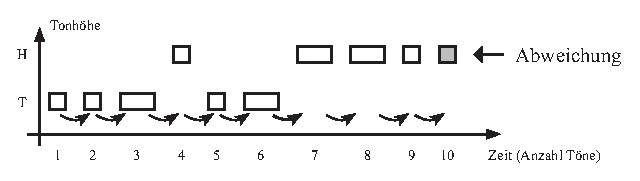
\includegraphics[width=\textwidth]{abb2-tones.eps}
    \end{minipage}}
    \vspace{10pt}
    \caption[Beispiel für eine Tonsequenz]{Beispiel für eine Tonsequenz. Die Länge des einen Tons sagt die Höhe des nächsten Tons vorher. In diesem Beispiel folgt auf einen kurzen Ton ein tiefer Ton (T) und auf einen langen Ton ein hoher Ton (H). Der letzte Ton ist im Beispiel von der Regel abweichend: Auf einen kurzen Ton (Ton 9) folgt kein tiefer Ton, wie die Regel es vorhersagen würde, sondern ein hoher Ton (Ton 10).}
    \label{stimuli}
  \end{minipage}
\end{figure}

Von den zwei Merkmalen (Höhe und Länge) ist dem Prinzip nach jeweils die Länge der entscheidende Prädiktor für das Merkmal Höhe des nächsten Tons. Während des Versuchs bekam die eine Hälfte der Probanden die eine Regel, die anderen Hälfte die andere Regel präsentiert. Um die MMN auszulösen wurde die Regel an vereinzelten Stellen unterbrochen. Eine Beispielsequenz dieser Regel ist in Abbildung \ref{stimuli} gezeigt.\\
Alle Probanden durchliefen in gegebener Reihenfolge außerdem folgende Bedingungen:

\begin{compactitem}
  \item \textbf{Ignore}: Die Probanden schauten einen Stummfilm mit Untertiteln und sollten weder auf die Töne reagieren, noch darauf achten.
  \item \textbf{Implicit detection}: Den Probanden wurde die Regel nicht erklärt, sie sollten jedoch eine Taste drücken, wenn sie das Gefühl hätten, dass ein Ton nicht passt.
  \item \textbf{Explicit detection}: Den Probanden wurde die Regel erklärt (mit Hilfe eines Schaubildes), sie sollten eine Taste drücken, wenn sie der Meinung waren, dass einer der Töne nicht in die Regel passt.
\end{compactitem}

Im Ergebnis zeigte sich, dass unter allen drei Bedingungen ein signifikanter Ausschlag der MMN vorlag, sofern eine Abweichung vorkam. Es zeigte sich allerdings auch, dass sich der Ausschlag der MMN in allen drei Fällen nicht signifikant voneinander unterschied. Es war also unerheblich, ob die Probanden die Töne ignorierten, intuitiv darauf reagierten oder aktiv und bewusst darauf achteten. Eine intuitive oder bewusste Übung konnte die Erkennungsleistung des Gehirns nicht steigern. Demzufolge waren implizite ebenso wie explizite Lernprozesse auf der Ebene neuronaler Signale anscheinend nicht vorhanden. Für einen - zumindest kleinen - Lerneffekt spricht hingegen, dass die behavioralen Daten in den zwei detection-Bedingungen in Form der Erfolgsrate beim Drücken der Tasten signifikant vom Zufall abwichen, wenn auch nur sehr gering. Qualitativ wurde außerdem berichtet, dass die Probanden das Wissen über die Regel nur als wenig hilfreich einschätzten.\\
Aus den Ergebnissen haben \textcite{paavilainen2007preattentive} geschlossen, dass die Verarbeitung wohl überwiegend automatisiert und die Treffer in der explicit detection Bedingung eher auf Intuition, als auf explizites Wissen über die Regel zurückzuführen sind. Allerdings scheint sich die  Leistungsfähigkeit geringfügig verbessern zu können. Dies schlägt sich zumindest in der knapp überzufälligen behavioralen Erfolgsrate nieder. Letztlich war ein weiteres EKP, die so genannte P3, nicht ausgeprägt. Diese Komponente schlägt üblicherweise aus, wenn Stimuli bewusst klassifiziert werden. Die These, dass die Stimuli automatisiert und unbewusst verarbeitet werden, konnte damit bestätigt werden.

Die Studie von \textcite{paavilainen2007preattentive} wurde 1 Jahr später von \textcite{bendixen2008rapid} repliziert und erweitert. Dabei wurden die gleichen Regeln verwendet, auch Tonhöhe und Frequenz entsprachen den vorigen.\\
Die Regeln wurden in unterschiedlich langen Sequenzen (4, 9, 14, 19 Töne) regelkonform präsentiert und anschließend durch irreguläre Sequenzen (4-8 Töne) unterbrochen. Diese Unterbrechung führt dazu, dass das Gehirn immer wieder von vorne beginnen muss, eine Regel zu erkennen, zumal nach einer irregulären Sequenz auch die reguläre Sequenz variieren kann, da wie oben beschrieben, zwei solcher regulären Regeln existieren. Es wurde zwischen zwei Bedingungen unterschieden:

\begin{compactitem}
  \item \textbf{Passiv}: Kontinuierliche Stimulus-Präsentation, wobei die Probanden einen Stummfilm schauten und die Stimuli ignorieren sollten.
  \item \textbf{Aktiv}: Probanden hörten abgegrenzte Sequenzen unterschiedlicher Länge, wobei der letzte Ton Standard oder Deviant sein konnte. Sie bekamen die Regeln erklärt und sollten per Tastendruck reagieren.
\end{compactitem}

Die Probanden bekamen erst 8 Blöcke in der Passiv-Bedingung präsentiert und wurden gefragt, ob sie eine Regel erkannten. Anschließend bekamen sie 5 weitere Blöcke in der Aktiv-Bedingung präsentiert. In keinem Fall erkannten die Probanden die Regel nach der Passiv-Bedingung korrekt, sofern sie überhaupt eine erkannten. Der Sensitivitätsindex (d-prime) lag noch signifikant über dem Zufallsniveau, sowohl für kurze (5 und 10 Töne), als auch für lange (15 und 20 Töne) Sequenzen. Die MMN zeigte jedoch nur für lange Sequenzen eine signifikante Ausprägung.\\
Die Ergebnisse von \textcite{paavilainen2007preattentive} konnten damit zum einen bestätigt werden, zum anderen konnte gezeigt werden, dass für die Regelerkennung zunächst einige Stimuli nötig sind, bis das Gehirn die entsprechende Regel abgeleitet hat. Allgemein liegt ein kontinuierlicher Zusammenhang vor: Je mehr regelkonforme Stimuli zuvor präsentiert werden, desto höher ist der Ausschlag der MMN bei einer Unterbrechung. Es scheint also eine Akkumulation abzulaufen, die Hinweise auf eine Regel ansammelt. Entscheidend ist jedoch, dass auch in dieser Studie das bewusste Erkennen einer Regelverletzung nicht möglich war. Auch hier zeigte sich die Abwesenheit der P3-Komponente und damit die Abwesenheit bewusster Klassifikationsprozesse.

\subsection{Lernen prozeduralen Wissens}

Zusammenfassend liegt also bezüglich der Erkennung komplexer Regeln eine automatisierte und unbewusste Verarbeitung vor. Während auf neuronaler Ebene Abweicher von der Regeln zuverlässig erkannt werden, ist es dem Menschen nicht möglich, diese Regeln bewusst anzuwenden bzw. Regelabweichungen zu erkennen. Da Lernen - kurz gefasst - als eine relativ stabile Veränderung des Verhaltens, Denkens oder Fühlens definiert wird, kann davon ausgegangen werden, dass ein Lernprozess an dieser Stelle nicht stattfindet. Eine Verhaltensänderung konnte nicht oder nur in sehr geringem Maße beobachtet werden. Für eine weitere Untersuchung ist es demnach zunächst von Bedeutung zu betrachten, wie das implizite und explizite prozedurale Lernen funktioniert. Aus bestehenden Theorien über das Lernen kann abgeleitet werden, wie ein expliziter prozeduraler Lernprozess komplexer Regeln gestaltet werden könnte. Ziel ist es, einen solchen Lernprozess zu gestalten, um zu zeigen, dass ein explizites Lernen prinzipiell möglich ist. Sollte dieser Nachweis erfolgreich verlaufen, könnte dies ein Ansatz sein, um die Funktionsmechanismen hinter der Lücke zwischen der automatisierten unbewussten und der aktiven bewussten Verarbeitung zu verstehen.

Grundsätzlich lässt sich der Lernprozess als prozedurales Lernen (abgegrenzt von deklarativem Lernen) klassifizieren, sofern das Drücken der Taste passend zu den Abweichern gelernt wird. Das Lernen deklarativen Wissens würde voraussetzen, dass es für die Erkennung reichen würde, das Wissen über die Regel zu kennen. Wie sich bisher gezeigt hat, scheint das reine Wissen jedoch nicht ausreichend zu sein. Das erworbene Wissen muss bei der Erkennung von Abweichungen in einen Handlungsprozess umgewandelt werden. Das prozedurale Lernen bezieht sich dabei weniger auf das Ausführen sichtbarer Handlungen, sondern vielmehr auf das Lernen einer Abfolge unterschiedlicher Verarbeitungsschritte.\\
In den bisherigen Untersuchungen lag – wenn überhaupt – nur implizites Lernen vor. Interessant wäre also zu betrachten, wie explizites Lernen erreicht werden kann, das den Probanden bisher nicht möglich war. Es ist auf Grund der genannten Ergebnisse davon auszugehen, dass sich ein expliziter Lernprozess relativ schwierig gestalten könnte.

Die Klassifikation in prozedurale Prozesse macht nun deutlich, dass ein einfaches Zeigen der Regel (z.B. an einem Schaubild) kaum ausreichen kann, um die Regel adäquat anzuwenden, zumal die Stimuli mit 50\,ms bzw. 150\,ms Länge und einem Inter-Stimulus-Intervall (ISI) von 300\,ms präsentiert wurden. Diese hohe Geschwindigkeit erfordert wahrscheinlich ein langes Training, sofern ein expliziter Prozess verlangt wird. \textcite{fitts1967human} gingen davon aus, dass prozedurales Wissen in drei aufeinander folgenden Schritte gelernt werden kann:

\begin{compactenum}
  \item \textbf{Kognitives Stadium}: In diesem Stadium handelt es sich noch um eine deklarative Repräsentation. Das deklarative Wissen kann in bestehendes Wissen integriert und mit diesem verknüpft werden. Eine Vermittlung sollte präzise und verständlich erfolgen. Angewendet werden kann z.B. ein Schaubild.
  \item \textbf{Assoziatives Stadium}: Eine prozedurale Repräsentation wird aufgebaut. Es entwickeln sich Wenn-Dann-Regeln. Sofern ein bestimmtes Ereignis eintritt, wird automatisch eine spezifische Reaktion ausgeführt. Dieses Stadium kann vor allem durch regelmäßige Übung erreicht werden. Wichtig ist hier auch das Geben von Feedback.
  \item \textbf{Autonomes Stadium}: Das prozedurale Wissen kann schnell und automatisiert abgerufen werden. Die einzelnen Repräsentationen sind stabil miteinander verbunden und führen zu einer fehlerfreien Ausführung. Der Ressourcenaufwand minimiert sich. Erreicht wird dies durch das Praktizieren über längere Zeiträume.
\end{compactenum}

Eine gute Beschreibung des prozeduralen Lernens bietet auch der Learning Cycle von \textcite{whitmore2009coaching}. Der Kreislauf teilt das Lernen in 4 aufeinanderfolgende Schritte ein:

\begin{compactenum}
  \item \textbf{Unconscious incompetence}: Kein Verständnis vorhanden.
  \item \textbf{Conscious incompetence}: Es liegt zwar nur eine geringe Performanz vor, Fehler und Schwächen werden jedoch bemerkt und können korrigiert werden.
  \item \textbf{Conscious competence}: Die Leistung verbessert sich, zur Durchführung ist jedoch ein hoher kognitiver Aufwand nötig.
  \item \textbf{Unconscious competence}: Es liegt eine hohe Performanz vor, der kognitive Aufwand verringert sich deutlich zugunsten automatisierter Abläufe.
\end{compactenum}

Warum explizites Lernen in den vorigen Studien \parencites{bendixen2008rapid}{paavilainen2007preattentive} nicht oder nur in sehr geringem Umfang möglich war, kann nun auf Basis der beiden Modelle gut erklärt werden. Unter der Voraussetzung, dass prozedurales Wissen vorliegt und gelernt werden muss, wurde in beiden Studien lediglich das kognitive Stadium erreicht \parencite[nach][]{fitts1967human}. Bei \textcite{bendixen2008rapid} wurde kein langsamer Übungsblock vorgenommen. Die Wahrscheinlichkeit, dass stabile Wenn-Dann-Regeln aufgebaut werden konnten, ist in diesem Fall eher gering, da die Probanden vermutlich auf Grund der Überforderung keine Möglichkeit hatten, ihr Verhalten adäquat zu überdenken. In beiden Studien wurde kein Feedback gegeben, und der Schwierigkeitsgrad stieg vermutlich ebenfalls bei beiden Studien zu abrupt an. Bei \textcite{paavilainen2007preattentive} wurde von einem ISI von 2000\,ms in der Übung direkt auf 300\,ms in der Anwendung erhöht, bei \textcite{bendixen2008rapid} wurde direkt mit einem ISI von 300\,ms begonnen. Nach der Annahme der Zone proximaler Entwicklung von Wygotski \parencite{kozulin2003vygotsky} sollte der nächste Lernschritt knapp über dem aktuellen Lernniveau sein, um ein optimales Lernen zu gewährleisten. Diese Voraussetzung wurde in beiden Experimenten nicht hinreichend erfüllt.\\
Nach dem Modell von \textcite{whitmore2009coaching} dürften die Probanden nicht über die zweite Stufe hinaus gekommen sein, bei \textcite{bendixen2008rapid} vermutlich nicht über die erste, da Fehler und Schwächen auf Grund des schnellen Einstiegs und des fehlenden Feedbacks nicht bemerkt werden können. Die Theorie liefert an dieser Stelle eine gute Erklärung für das schlechte Abschneiden der Probanden bei den expliziten Aufgaben in den vorangegangenen Experimenten.

\subsection{Hypothese}

An dieser Stelle soll zunächst noch einmal der aktuelle Kenntnisstand zur Regelerkennung und zur Detektion von Fehlern zusammengefasst werden:

\begin{compactitem}
\item Der Mensch besitzt die Fähigkeit, hochautomatisiert und daher mit hoher Geschwindigkeit und Präzision Regeln zu erkennen (angezeigt durch die MMN).
\item Diese Fähigkeit funktioniert insbesondere auch für komplexe Regeln und ohne bewusste Aufmerksamkeit.
\item Das bewusste Lernen und der bewusste Zugriff auf diese Regeln ist sehr schwer.
\item Die aktive bewusste und die automatisierte unbewusste Verarbeitung basieren vermutlich auf unterschiedlichen Verarbeitungsprozessen. Die automatisierte Verarbeitung wird bereits auf sensorischer Ebene vermutet.
\end{compactitem}

Um die Unterschiede zwischen den Verarbeitungsmechanismen verstehen zu können ist es nötig, die bisherigen Erkenntnisse in einzelne Schritte zu segmentieren. Ein erster Schritt wurde in diesem Experiment getestet. Dabei wurde die Frage gestellt, ob, und wenn ja unter welchen Umständen, explizites Lernen komplexer Regeln möglich ist. Dafür wurde folgende Hypothese formuliert:

\textbf{Hypothese}: Das Lernen der komplexen Regeln sollte unter Beachtung der Lerntheorien für prozedurales Wissen auch explizit möglich sein.

Während bisher die Regel einfach erklärt wurde, wird im Folgenden ein theoretisch abgeleitetes Lernkonzept angewendet. Dabei wird der Schwerpunkt auf der 3-stufigen Theorie von \textcite{fitts1967human} liegen. Beachtet werden soll außerdem die Zone proximaler Entwicklung. Im folgenden Methoden-Abschnitt wird die Hypothese unter Beachtung der Experimentalbedingungen noch einmal präzisiert.

\section{Methoden}

\subsection{Probanden}

Insgesamt wurden für die Untersuchung 19 Probanden getestet. Die Daten einer Person mussten wegen technischer Probleme während des Versuchsdurchgangs aus der Analyse genommen werden. Von den verbleibenden 18 Probanden waren 3 männlich (16.7\,\%) und 15 weiblich (83.3\,\%). Das Durchschnittsalter betrug 27 Jahre (SD~=~8), die Probanden waren zum Zeitpunkt des Experimentes zwischen 18 und 53 Jahre alt. Von den 18 Probanden fühlten sich 11 gut ausgeschlafen und 13 gut konzentriert. Die übrigen hatten mindestens mäßig geschlafen und waren mindestens mäßig konzentriert, entsprechend hatte kein Proband schlecht geschlafen oder war schlecht konzentriert. Im Selbstbericht gab keiner der Probanden an, im Voraus Substanzen zu sich genommen zu haben, die das Nervensystem hätten beeinträchtigen können, und alle Probanden gaben an, gut hören und den Experimentalbedingungen entsprechend ausreichend sehen zu können. Eine Versuchsperson musste auf Englisch instruiert werden, die Aufgabe wurde jedoch ohne Schwierigkeiten verstanden.

\subsection{Versuchsaufbau}

In Abbildung \ref{experiment} ist eine Skizze des Versuchsaufbaus gezeigt. Das Experiment musste in einer nicht ganz optimalen Experimentalumgebung durchgeführt werden, da sich die Labore der Professur für Kognitive einschließlich Biologische Psychologie zum Erhebungszeitpunkt gerade im Umbau befanden. Um trotzdem möglichst optimale Bedingungen zu erhalten, wurde versucht, möglichst viele eventuell störende Faktoren konstant zu halten.

\begin{wrapfigure}{r}{.6\textwidth}
  \centering
  \begin{minipage}{.55\textwidth}
    \setlength{\fboxsep}{.05\textwidth}
    \fbox{\begin{minipage}{.95\textwidth}
      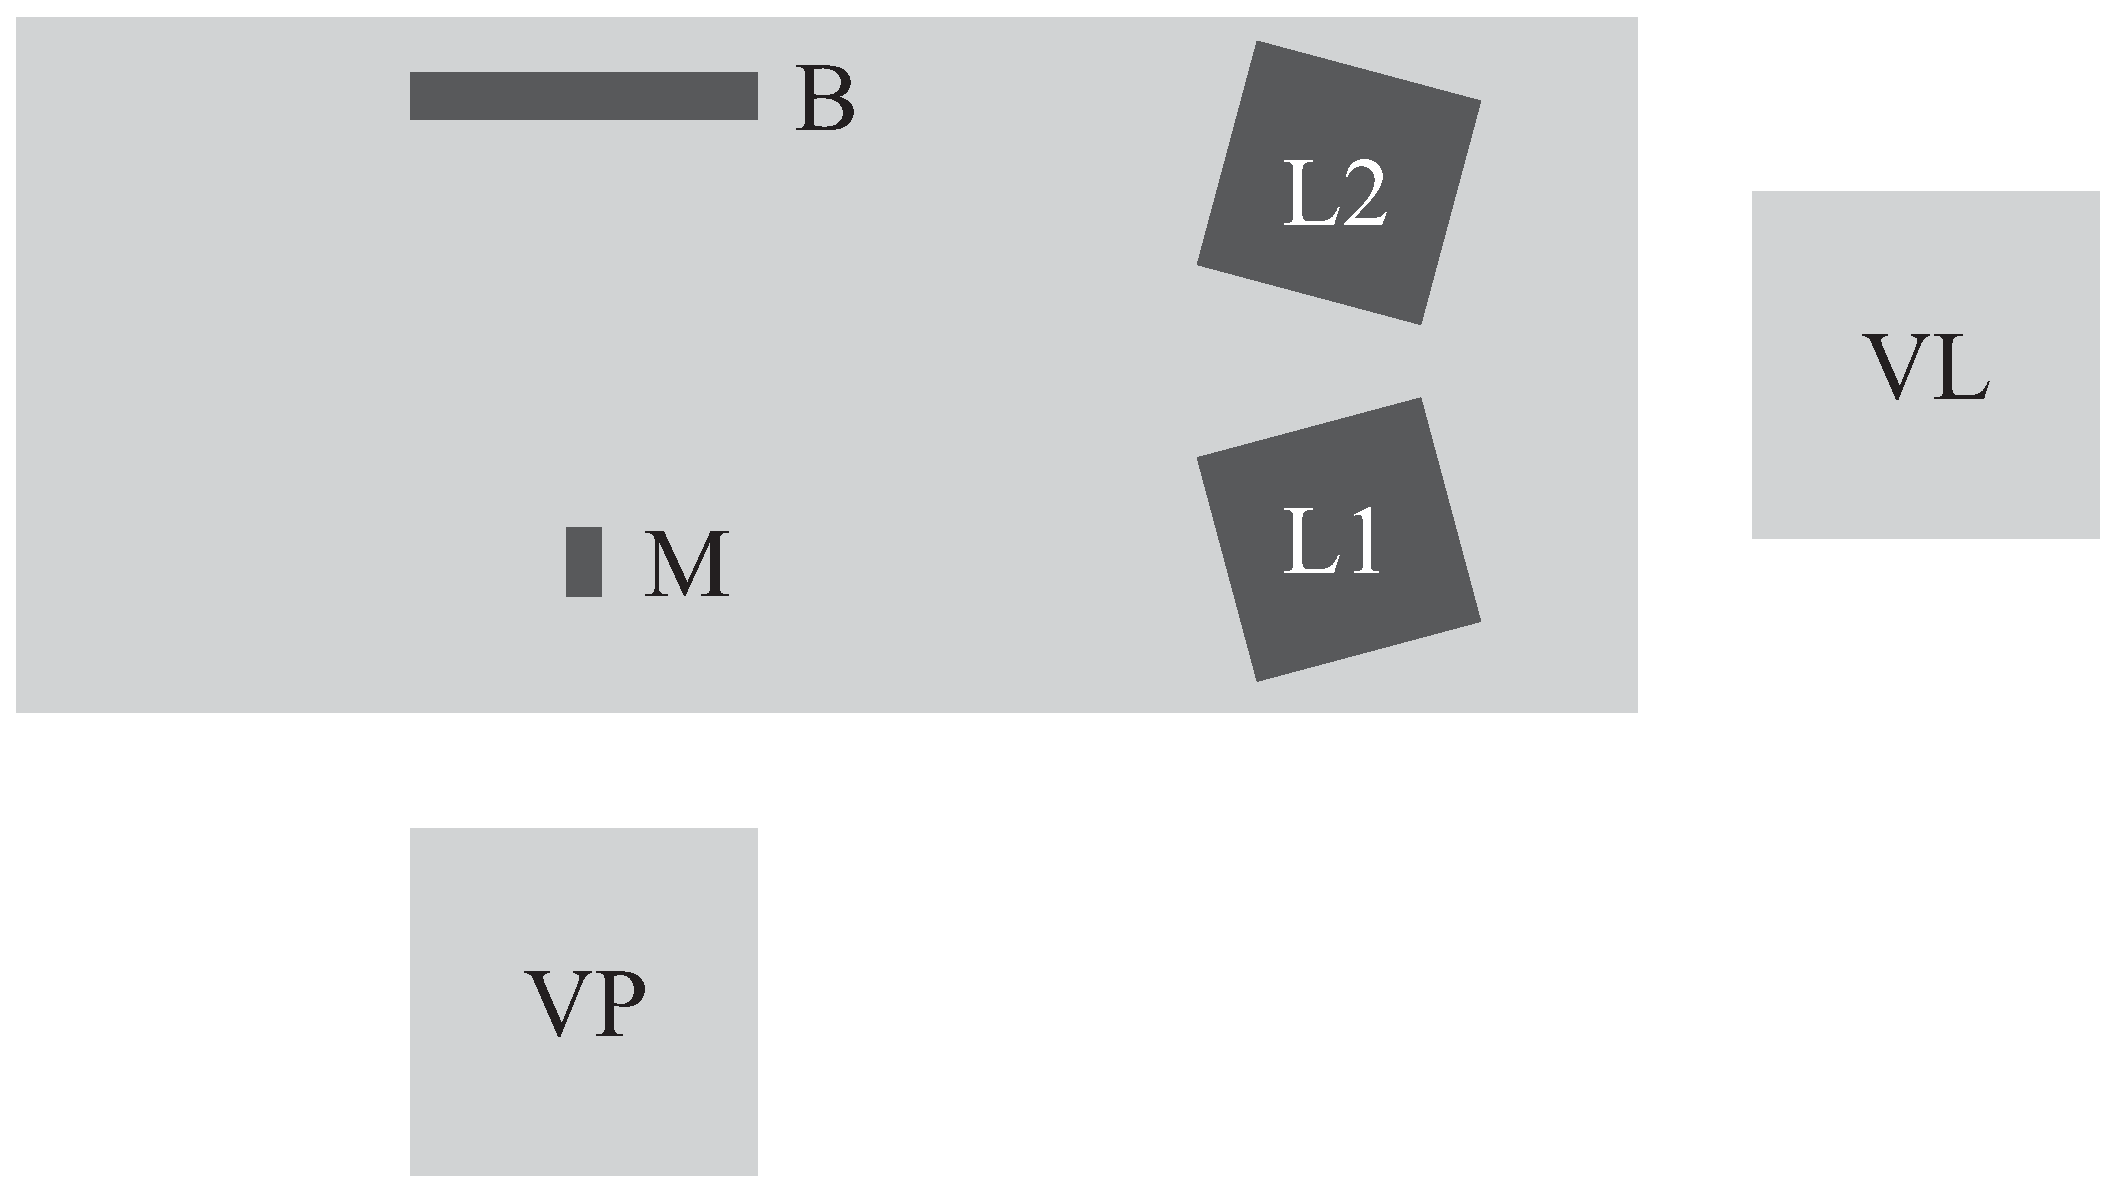
\includegraphics[width=\textwidth]{abb1-versuchsaufbau.eps}
    \end{minipage}}
    \vspace{10pt}
    \caption[Aufbau des Experimentes]{Aufbau des Experimentes. Laptop 1 (L1) mit Programm für Experiment und Laptop 2 (L2) für Versuchsleiter (VL). Bildschirm (B), Maus (M) und Kopfhörer (nicht eingezeichnet) für Versuchsperson (VP).}
    \label{experiment}
  \end{minipage}
\end{wrapfigure}

Auf Laptop 1 (L1) wurde das Programm für den Versuch\footnote{\label{foot:1}Der Programmcode für den Versuch wurde in einer Vorversion von Prof. Dr. Alexandra Bendixen zur Verfügung gestellt.} ausgeführt, dieser wurde vom Versuchsleiter (VL) bedient. Für das Abspielen der Töne und das Speichern der Reaktionsdaten wurde das Programm Matlab verwendet. Der Laptop (L1) war an den Bildschirm (B) angeschlossen, welcher der Versuchsperson (VP) zur Verfügung stand. Auf diesem Bildschirm wurde angezeigt, wann die Versuchsperson reagieren sollte. Dafür stand der Versuchsperson eine Computer-Maus (M) mit 2 Tasten zur Verfügung. Während in den bisherigen Experimenten auch immer eine EEG-Messung durchgeführt wurde, beschränkte sich dieses Experiment auf Reaktionsdaten (d-prime und Reaktionszeit). Des Weiteren wurde ein zweiter Laptop (L2) verwendet, damit der Versuchsleiter (VL) die Versuchsperson während der Blöcke nicht störte. Unter Experimentalbedingungen im Labor sind Versuchsleiter und Versuchsperson räumlich getrennt. In diesem Fall war eine räumliche Trennung nicht möglich. Um etwaige Versuchsleitereffekte zu minimieren, sollte der Versuchsleiter nicht den Eindruck vermitteln, die Versuchsperson zu beobachten oder gar zu kontrollieren. Auch subtile Reaktionen des Versuchsleiters auf eventuelles gutes oder schlechtes Abschneiden der Versuchsperson sollten vermieden werden. Dafür wurde zusätzlich zu der Verwendung von L2 der Bildschirm von L1 maximal abgedunkelt und nach Möglichkeit vom Versuchsleiter während der Stimulus-Präsentation nicht beachtete. Die Ablenkung an L2 erfolgte durch kognitiv anstrengende Aufgaben. Dabei wurde sichergestellt, dass der Versuchsleiter nach dem Ende eines Blockes unverzüglich wieder zur Versuchsperson umschaltete. Die Versuchsperson musste nach Beendigung eines Blockes sofort und direkt die volle Aufmerksamkeit bekommen, um die Motivation aufrecht zu erhalten.

Um Störungen zu verhindern und die Experimentalbedingungen möglichst optimal zu halten, wurde durch anbringen eines Schildes sichergestellt, dass während des Versuchs keine dritte Person in den Raum kam. Außerdem wurde das Fenster geschlossen. Die Kopfhörer wurden vorher auf eine normierte Lautstärke eingestellt. Der Bildschirm (B) war zunächst ausgeschaltet und wurde erst unmittelbar vor dem Start des Versuchs eingeschaltet.

\subsection{Stimuli}

Innerhalb der Blöcke bekam die Versuchsperson auditive Stimuli präsentiert. Diese bestanden aus Tonsequenzen à 11, 16 oder 21 Tönen. Der erste Ton wurde zufällig gewählt, alle folgenden wurden entsprechend der Regel gestaltet. Somit ergaben sich im Standard-Fall 10, 15 oder 20 regelkonforme Töne innerhalb einer Sequenz. Dabei entsprachen die Töne und die Regel denen bei \textcite{paavilainen2007preattentive}. Die Töne unterschieden sich in Höhe (hoch/tief) und Länge (kurz/lang). Dabei wurden die Frequenzen für hohe (1500\,Hz) und tiefe (1000\,Hz) Töne wie zuvor verwendet. Auch die Länge der Töne blieb mit 50\,ms für kurze und 150\,ms für lange Töne identisch zu den vorigen Experimenten. Die Regel für die Töne lautete wie in der Einleitung beschrieben:

\begin{compactitem}
  \item Auf einen langen Ton folgt ein hoher Ton, auf einen kurzen Ton folgt ein tiefer
Ton
  \item Auf einen langen Ton folgt ein tiefer Ton, auf einen kurzen Ton folgt ein hoher
Ton
\end{compactitem}

Unterschiede zu den vorherigen Experimenten gab es bei der Wahl des Inter-Stimulus-Intervalls (ISI), welches zwischen den Blöcken variierte. Angewendet wurden Intervalle von 300\,ms, 600\,ms und 900\,ms. Der letzte Ton bildete außerdem in 50\% der Fälle eine Ausnahme und wich von der gegebenen Regel ab. Dabei wurden die Sequenzen nicht kontinuierlich präsentiert. Die nächste Sequenz startete erst, nachdem ein Tastendruck ausgeführt wurde. Hierfür hatten die Probanden beliebig viel Zeit, wurden jedoch angehalten, relativ zügig zu reagieren. In Abbildung \ref{stimuli} in der Einleitung ist eine Beispielsequenz mit einer Abweichung am Ende skizziert.\\
Die jeweilige Versuchsperson sollte mit der Maus nun darauf reagieren und entscheiden, ob der letzte Ton passend oder abweichend ist. Dem zufolge liegt die Leistung der Versuchsperson darin, zunächst die Regel zu erkennen und nach Beendigung der Sequenz eine Entscheidung zu treffen. Auf dem Bildschirm war während der Sequenzen ein Fixationskreuz zu sehen, welches unmittelbar nach dem letzten Ton der Sequenz in ein Fragezeichen wechselte. Da die Sequenzen unterschiedlich lang waren, sollte dieses Hilfsmittel die Unsicherheitszeit zwischen den Sequenzen, die mindestens dem Inter-Stimulus-Intervall entsprach, möglichst gering halten. Eine systematische Reaktionszeit-Variation zwischen den Blöcken sollte damit vermieden werden.

\subsection{Ablauf}

Der Ablauf des Experimentes erfolgte nach einer standardisierten Checkliste. Damit konnte der Versuchsleiter überprüfen, ob nach jedem Schritt alle relevanten Punkte erläutert wurden. Die Liste war für die Versuchsperson nicht sichtbar. Folgender Ablauf wurde durchgeführt:

\begin{compactenum}
  \setcounter{enumi}{-1}
  \item \textbf{Vorbereitung}: Präparation des Versuchsraumes (vor dem Eintreffen der VP)
  \item \textbf{Einführung}: Erklärung des Experimentes
  \item \textbf{Block 1 (schnell)}: Durchgang mit ISI von 300\,ms
  \item \textbf{Arbeitsblatt}: Lernen der Regel mit Hilfe eines Arbeitsblattes
  \item \textbf{Block 2 (langsam)}: Durchgang mit ISI von 900\,ms und Feedback
  \item \textbf{Block 3 (mittel)}: Durchgang mit ISI von 600\,ms und Feedback
  \item \textbf{Block 4 (schnell)}: Durchgang mit ISI von 300\,ms
  \item \textbf{Nachbereitung}: Musikfragebogen, Datensicherung
\end{compactenum}

Die Variation der ISI zwischen den Blöcken ist, ebenso wie das Arbeitsblatt, ein Lernprozess im Sinne der Lerntheorie von \textcite{fitts1967human}. Dabei repräsentiert das Arbeitsblatt das kognitive Stadium mit einem Übergang in das assoziative Stadium. Block~2 und Block~3 bildeten das assoziative Stadium und sollten im Idealfall in Block~4 in das autonome Stadium überführen.

\subsubsection{(1) Einführung}

Nach dem Unterschreiben der Formulare wurden die Rahmenbedingungen des Experimentes erklärt. Dabei wurde beim ersten Durchgang noch nicht die Regel erklärt. Der erste Durchgang diente als Kontrolldurchgang. Der Versuchsperson wurde folgendes erläutert:

\begin{compactitem}
\item Eine Sequenz besteht aus 10-20 Tönen
\item Ein Block besteht aus 24 Sequenzen
\item Die Töne unterscheiden sich in Höhe (hoch/tief) und Länge (kurz/lang)
\item Der letzte Ton einer Sequenz kann zu den vorigen passen oder nicht passen
\item Eine Maustaste für "passt", eine für "passt nicht"
\item Erster Durchgang wird intuitiv gelöst
\end{compactitem}

Ergänzend erklärt wurde außerdem, dass der Versuchsleiter während der Blöcke keine Ergebnisse beobachtet und sich an Laptop~2 ablenken wird. Außerdem wurde der Versuchsperson verdeutlicht, dass Genauigkeit wichtig ist. Letztlich bekam die Versuchsperson noch die Empfehlung, den rechten und linken Zeigefinger jeder Hand pro Taste zu verwenden, um rechts-links Schwierigkeiten zu vermeiden. Die Tastenbelegung der Maus variierte zwischen den Versuchspersonen gleichmäßig, um eventuelle Effekte von Händigkeit auszuschließen. Die Versuchsperson bekam die Tastenbelegung vor jedem Block auf einem Startbildschirm angezeigt.

\subsubsection{(2) Block 1}

In Block~1 wurde zunächst ein Inter-Stimulus-Intervall von 300\,ms verwendet. Dies entspricht dem ISI von \textcite{paavilainen2007preattentive} und \textcite{bendixen2008rapid}. Nachdem der erste Block beendet war, wurde die Versuchsperson gefragt, ob sie eine Regel erkannt hatte. Sofern die Versuchsperson dies verneinte oder keine korrekte Regel nannte, wurde die Versuchsperson durch den Versuchsleiter ermutigt mit der Aussage, dass noch niemand jemals zu diesem Zeitpunkt eine Regel erkannt habe und das Nicht-Erkennen der Regel ein wichtiger Bestandteil des Experimentes sei.

\subsubsection{(3) Arbeitsblatt}

In diesem Schritt, unmittelbar nach Block~1, wurde der Versuchsperson ein Arbeitsblatt (siehe Anhang) gegeben. Dafür setzte sich der Versuchsleiter neben die Versuchsperson an die lange Kante des Tisches neben Position VP (siehe Abbildung~\ref{experiment}). Das Arbeitsblatt wurde in allen Fällen gemeinsam bearbeitet. Dabei wurde zunächst anschaulich die Regel erklärt. Anschließend war die Versuchsperson aufgefordert, für beide Regeln je eine eigene Sequenz zu erfinden und zu zeichnen. Bis zu diesem Punkt handelte es sich noch um die kognitive Stufe. Auf der letzten Seite des Arbeitsblattes wurde dann in die assoziative Stufe gewechselt. Dort waren Sequenzen vorgegeben, bei denen bestimmt werden musste, ob der letzte Ton regelkonform oder abweichend ist. Diese Übung entsprach in visuell/bildlicher Form der auditiven Übung und sollte der Festigung der verstandenen Regel dienen. Nach Beendigung des Arbeitsblattes wurde dieses für die Versuchsperson unzugänglich abgelegt, um gleiche Bedingungen für alle Versuchspersonen zu schaffen und eine Zuhilfenahme der Arbeitsblatt-Unterlagen generell auszuschließen. Im Anschluss wurde der Versuchsperson das weitere Vorgehen erläutert. Dabei wurde die Versuchsperson explizit darauf vorbereitet, dass die Regelerkennung bzw. das Erkennen eines Abweichers im auditiven Experiment deutlich schwieriger ist als auf dem Blatt, um eine Verringerung der Motivation möglichst zu vermeiden.

\subsubsection{(4) Block 2}

Block~2 erfolgte mit einem ISI von 900\,ms. Block~2 war damit der langsamste Block und sollte einen geeigneten Übergang von der Arbeitsblatt-Übung zu der auditiven Übung ermöglichen. Zur Unterstützung des Lernens wurde nach jedem Tastendruck ein kurzes Feedback angezeigt, ob die Sequenz richtig oder falsch beurteilt worden war. Nach Block~2 wurde die Versuchsperson kurz offen befragt (z.B. "Wie war es?"). Relevante Antworten wurden notiert. Der Versuchsperson wurde eine kurze Pause angeboten.

\subsubsection{(5) Block 3}

Block~3 erfolgte analog zu Block~2, jedoch mit einem ISI von 600\,ms. Block~3 sollte das Gelernte weiter festigen.

\subsubsection{(6) Block 4}

In Block~4 wurde das ISI wieder auf die ursprünglichen 300\,ms gestellt. In diesem Block wurde der Versuchsperson kein Feedback mehr gegeben, da an diesem Punkt davon ausgegangen wurde, dass die Versuchsperson bereits das autonome Stadium erreicht hat.

\subsubsection{(7) Nachbereitung}

Nach Block~4 wurde die Versuchsperson noch ein letztes Mal offen über den Versuch befragt. Es wurden letzte Formalien geklärt und ein Fragebogen zur Musikalität ausgefüllt (siehe Anhang). Nach der Verabschiedung der Versuchsperson wurden alle Daten gesichert.

Die Hypothese, die in der Einleitung formuliert worden war, lässt sich an dieser Stelle anhand des konkreten Experimentes präzisieren. Wenn ein expliziter Lernprozess prozeduralen Wissens nach der Lerntheorie möglich ist, dann sollte die Leistung in der Erkennung der von der Regel abweichenden Töne am Ende der Sequenzen in Block~4 signifikant von der in Block~1 bzw. vom Zufall abweichen.

\section{Ergebnisse}

Im Ergebnis hatten zwar ein paar Versuchspersonen nach dem ersten Block (Schritt~2) vermeintlich eine Regel erkannt, meist konnte diese aber nicht präzise konkretisiert werden. Die erkannten Muster entsprachen zudem in keinem Fall der tatsächlichen Regel.

\begin{figure}[b]
  \centering
  \begin{minipage}{\textwidth}
    \fbox{\begin{minipage}{\textwidth}
      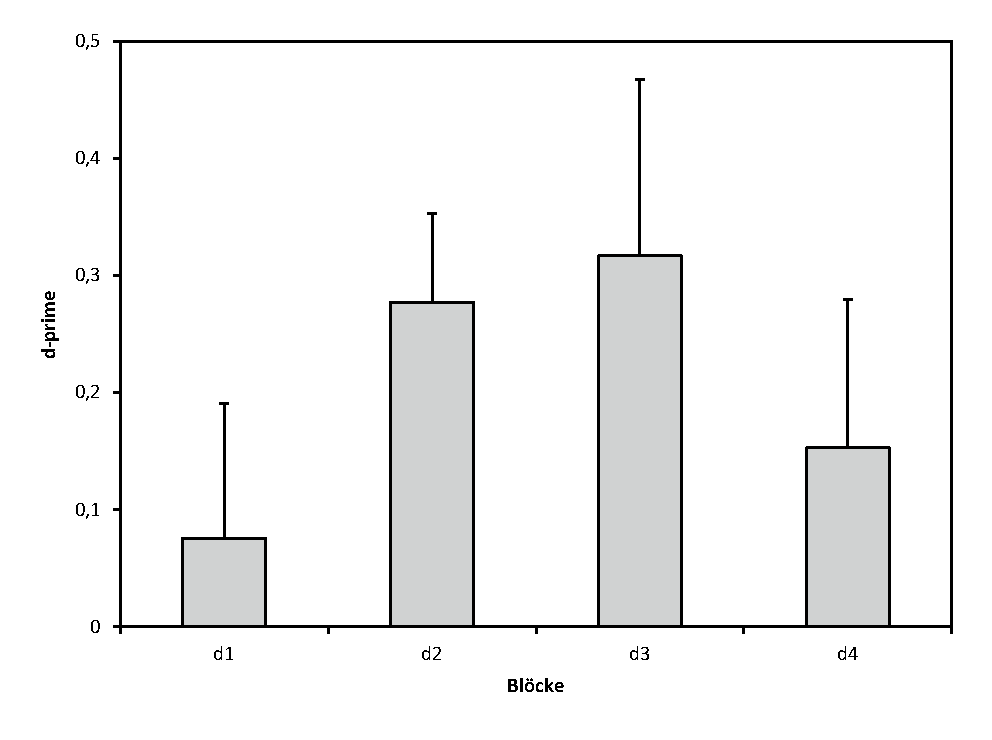
\includegraphics[width=\textwidth]{abb3-dprime.eps}
    \end{minipage}}
    \vspace{10pt}
    \caption[Mittelwerte der Sensitivitätsindizes]{Mittelwerte der Sensitivitätsindizes über alle 18 Versuchspersonen in den Blöcken 1 - 4 mit Standardfehler.}
    \label{dprime}
  \end{minipage}
\end{figure}

Nach der Erläuterung der Regel (Schritt~3) hatten alle Versuchspersonen die Aufgabe verstanden und die letzten Übungen auf dem Arbeitsblatt immer selbstständig gelöst. Sehr oft wurde dann im Verlauf des Experimentes berichtet, dass das Arbeitsblatt zwar das Verständnis ermöglicht habe, das Lösen der auditiven Übung jedoch trotzdem sehr schwer gewesen sei.

\begin{figure}[t]
  \centering
  \begin{minipage}{\textwidth}
  	%\setlength{\fboxsep}{.05\textwidth}
    \fbox{\begin{minipage}{0.47\textwidth}
      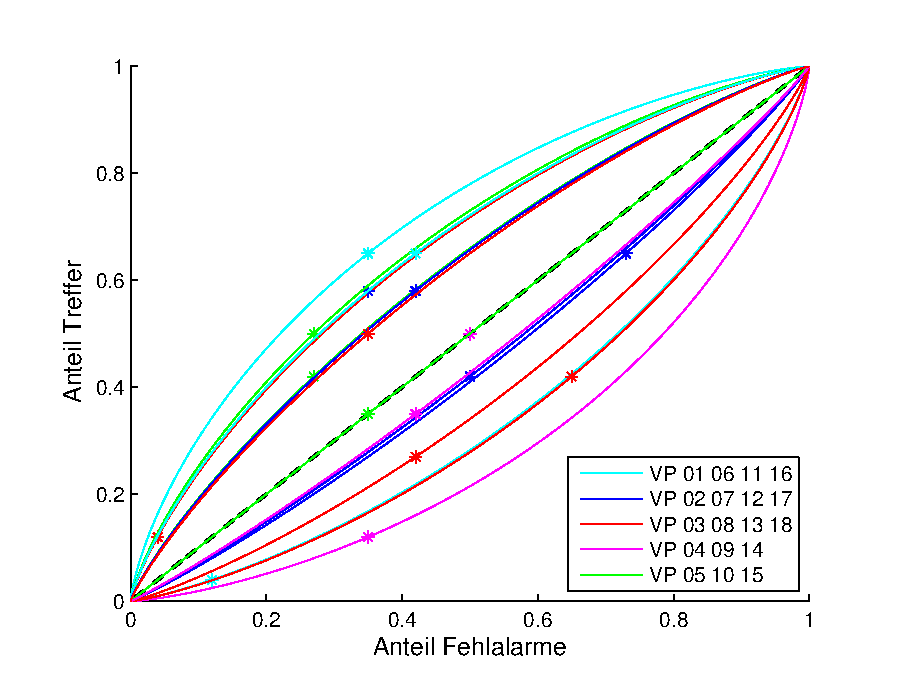
\includegraphics[width=\textwidth]{abb-roc-block1.eps}
    \end{minipage}}
    \hspace{0.02\textwidth}
    \fbox{\begin{minipage}{0.47\textwidth}
      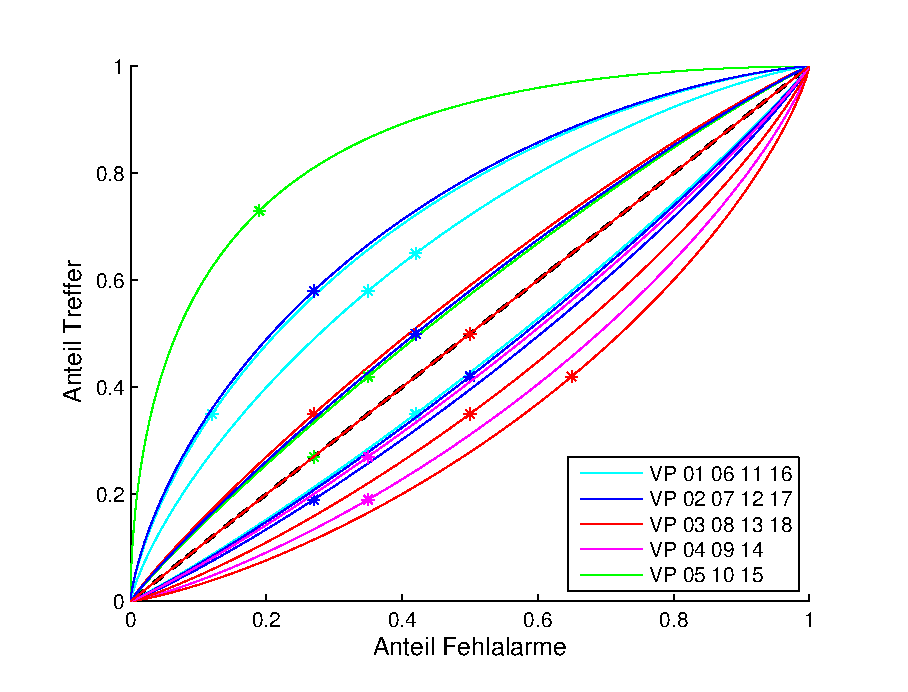
\includegraphics[width=\textwidth]{abb-roc-block4.eps}
    \end{minipage}}
    \vspace{10pt}
    \caption[Receiver Operating Characteristic Kurven]{Richtig-Positiv-Rate und Falsch-Negativ-Rate der Versuchspersonen für Block 1 (links) und Block 4 (rechts), dargestellt jeweils in ROC-Kurven (Receiver Operating Characteristic).}
    \label{roc}
  \end{minipage}
\end{figure}

Die Richtig-Positiv-Rate (hit rate) lag in Block 1 bei 40.74\,\%, die Falsch-Negativ-Rate (false alarm rate) bei 37.04\,\%. In Block 4 lag die Richtig-Positiv-Rate dann bei 41.67\,\%, die Falsch-Negativ-Rate bei 35.65\,\%. In Abbildung~\ref{dprime} ist der Sensitivitätsindex (d-prime) der 4 Blöcke abgebildet und in Abbildung~\ref{roc} ist die Verteilung der Richtig-Positiv-Raten und der Falsch-Negativ-Raten aller Versuchspersonen dargestellt. Von Bedeutung ist an dieser Stelle der d-prime der Blöcke 1 und 4, die Blöcke 2 und 3 dienten lediglich zur Übung. Blöcke 1 und 4 wurden beide mit einem ISI von 300\,ms und ohne Feedback präsentiert. Der erste Block wurde ohne das Regelwissen durchgeführt, der vierte Block nach Vermittlung des Wissens über die Regel und nach Übung der Erkennung von Regelabweichungen. Der Sensitivitätsindex in Block 1 beträgt d~=~0.076 (SE~=~0.115), in Block 4 liegt er bei d~=~0.153 (SE~=~0.126). Beide Werte unterscheiden sich nicht signifikant, t(17)~=~0.56, p~>~0.05. Auch wenn Block 4 gegen Null getestet wird, liegt der Sensitivitätsindex von Block 4 nicht signifikant über dem Zufallsniveau, t(17)~=~1.22, p~>~0.05.

\section{Diskussion}

Da sich der Sensitivitätsindex in Block 1 und Block 4 nicht unterscheiden, sprechen die Ergebnisse gegen einen expliziten Lerneffekt. Die qualitative Auswertung der Berichte der Versuchspersonen passen gut zu den Ergebnissen, denn auch die Versuchspersonen berichteten - vor allem im letzten Durchgang - konsistent von großen Schwierigkeiten beim Detektieren von Passenden und Abweichern am Ende der Sequenzen. Sie gaben an, meist intuitiv entschieden zu haben und vor allem in den schnellere Durchgängen oft nur geraten zu haben. Deutlich wird dieses Verhalten auch bei Betrachtung der ROC-Kurven in Abbildung~\ref{roc}.

Dies lässt zwei mögliche Schlussfolgerungen zu. Zum einen könnte dieser Aufgabentyp zu komplex sein, um ihn explizit und bewusst verarbeiten zu können. Die menschlichen Fähigkeiten wären in diesem Fall an ihren Grenzen. Zum anderen könnte aber auch der Lernprozess noch nicht ausreichend gestaltet worden sein. Für diese Annahme sprechen gleich mehrere Aspekte, die es lohnt zu betrachten. Möglich wäre, dass die Zone proximaler Entwicklung \parencite{kozulin2003vygotsky} nicht optimal gestaltet wurde. Die Lernmethodik wäre also auf Grund der hohen Komplexität immer noch zu schnell. In Abbildung~\ref{dprime} wird deutlich, dass die Sensitivität auch in den Blöcken~2 und~3 auf einem niedrigen Niveau liegt. Es wurde also auch in den einfacheren Übungsbedingungen - wenn überhaupt - nur sehr schwach gelernt. Eine Transferleistung des Lernens auf Block~4 ist nicht zu erwarten, wenn zuvor schon kaum erfolgreich gelernt wurde. Eine andere Option wäre, dass die Lernmodelle nicht zur Aufgabe passen. Entweder sind die Modelle nicht für das Lernen hoch komplexer Regeln ausgelegt oder die Klassifikation des Lernprozesses in prozedurales Wissen war nicht zutreffend. Um diese Optionen evaluieren zu können, werden im folgenden Kapitel `Post-Hoc-Analysen' einige weitere statistische Analysen durchgeführt. Diese gehen über die eigentliche Hypothese hinaus, können eventuell jedoch Hinweise liefern, die bei der Gestaltung zukünftiger Experimente helfen können. Ziel der folgenden Betrachtung sollte es sein, die vorliegenden Prozesse präziser zu klassifizieren und eine Systematik zur weiteren Untersuchung zu entwickeln.

\subsection{Sensorische Verarbeitung}

Die Ergebnisse stützen die Annahme von \textcite{paavilainen2007preattentive} und \textcite{bendixen2008rapid}, dass der Erkennungsprozess, der die MMN auslöst, im auditiven sensorischen Gedächtnis präattentiv abläuft. Weder ein expliziter, noch ein impliziter Lernerfolg konnte in diesem Experiment festgestellt werden, womit das Wirken höherer kognitiver Bereiche an dieser Stelle nicht anzunehmen ist. Unter der Annahme, dass die der MMN zugrunde liegenden Prozesse - auch wenn die MMN hier nicht erfasst wurde - vermutlich auch in diesem Experiment aufgetreten sind, kann geschlossen werden, dass nur sensorische Prozesse eine Erkennung derartig komplexer Aufgaben ermöglichen können.

\subsection{Phase der Gehirnoszillation}

Ein interessanter Ansatz, der in einem Review von \textcite{vanrullen2011ongoing} beschrieben ist, geht davon aus, dass Signale nur dann (bewusst) verarbeitet werden können, wenn sich das Gehirn gerade in einem bestimmten Oszillationszustand befindet. Der Oszillationszustand wird dabei mit Hilfe eines Elektroenzephalogramms (EEG) bestimmt und bezieht sich auf die Oszillation elektrischer Potentiale, welche durch die Rauschaktivität im Gehirn ausgelöst werden. Signale, die an der Wahrnehmungsschwelle liegen (d.\,h. einen Sensitivitätsindex von 0 besitzen), werden nur dann zuverlässig wahrgenommen, wenn das Signal auf eine aktive Oszillationsphase im Gehirn trifft. Da die Sensitivität auch in diesem Experiment nicht signifikant von Null abweicht und somit an der Wahrnehmungsschwelle liegt, könnten die von \textcite{vanrullen2011ongoing} beschriebenen Erkenntnisse eventuell auch bei der Erkennung von komplexen Regeln bzw. der Erkennung deren Abweichung ein Rolle spielen. Denkbar wäre, dass die letzten beiden Töne, die zum Abgleich der Regel im Gedächtnis behalten werden müssen, abhängig von der Phase der Oszillation im Gehirn gut oder weniger gut detektiert werden können. Wenn die Töne phasenverschoben eintreffen, wäre die Detektionsleistung nur eingeschränkt möglich. Treffen die Signale in Phase ein, dann dürfte die Detektionsleistung höher sein. In diesem Fall wäre die Aufgabe tatsächlich zu komplex und die menschlichen Fähigkeiten wären an ihren Grenzen.

\subsection{Lernbedingungen und Lernmethodik}

Offen bleibt an dieser Stelle, ob ein Lernprozess eventuell unter besseren Lernbedingungen und mit einer besseren Lernmethodik funktioniert hätte. Es gibt einige mögliche Ansätze um erklären zu können, warum der Lernprozess nicht erfolgreich war. Entsprechend können an dieser Stelle einige Optimierungsansätze formuliert werden.

\subsubsection{Lernbedingungen}

Die Untersuchungsbedingungen verliefen in keinem schalldichten, sondern unter eher provisorischen Bedingungen in einem für das Experiment präparierten Raum. Auch wenn Tür und Fenster immer geschlossen blieben, waren Geräusche von außen nicht gänzlich zu verhindern. Auch dass der Versuchsleiter im selben Raum anwesend war, könnte trotz der angewendeten Ablenkungsstrategie einen negativen Effekt auf die Versuchspersonen gehabt haben. Allein eine kleine Bewegung - sei es nur eine Veränderung der Sitzposition - könnte durch die Nähe schon eine Ablenkung bedeuten, zumal die Konzentrationsanforderungen bei dem Experiment für die Versuchspersonen enorm hoch waren. Unter optimalen Bedingungen sind Versuchsperson und Versuchsleiter während der Präsentation der Blöcke räumlich getrennt.

\subsubsection{Lernmethodik}

Ein anderer wichtiger Aspekt ist die Verbesserung der Lernmethodik. Der Lernaufwand wurde stark unterschätzt und der Lernprozess sollte deshalb noch deutlich umfassender gestaltet werden. Dazu könnten zum Beispiel weitere langsame Blöcke eingefügt, das Arbeitsblatt erweitert oder zusätzliche auditive Übungen durchgeführt werden.

Etwas ungünstig war ohnehin, dass es für den vierten Block keine Übung mit Feedback gab. Nach konsequenter Einhaltung der Lerntheorie hätte auch Block 4 noch einmal geübt werden müssen, um sicher zu gehen, dass dieser automatisiert ausgeführt werden kann. Man müsste genau genommen davon ausgehen, dass die Testdurchführung von Block 4 noch im assoziativen Stadium durchgeführt wurde und das autonome Stadium zuvor noch nicht erreicht wurde. Diese Vermutung geht direkt mit der bereits genannten Annahme einher, dass die Zone proximaler Entwicklung \parencite{kozulin2003vygotsky} nicht optimal angewendet wurde. Grundsätzlich ist jedoch - nicht zuletzt auch aufgrund der qualitativen Beurteilung - davon auszugehen, dass ein einfaches Einfügen eines weiteren schnellen Übungsblockes zu keiner nennenswerten Leistungssteigerung führen dürfte. Dafür sprechen auch die schwachen Ergebnisse in den Blöcken 2 und~3. Ein erfolgsversprechender Lernansatz müsste die Lernmethode von Beginn an deutlich erweitern. Nach jeder Geschwindigkeitsstufe müsste eine Erfolgssicherung stattfinden, analog des Verfahrens auf dem Arbeitsblatt. Dort wurde mit Hilfe der letzten Aufgabe sichergestellt, dass die Versuchsperson die Anwendung der Regel verstanden hat. Nach diesem Prinzip müsste auch im auditiven Experiment auf jeder Geschwindigkeitsstufe eine bestimmte Erfolgsrate gefordert sein, bevor die Versuchspersonen einen Block in der nächsthöheren Geschwindigkeitsstufe präsentiert bekommt.

Eventuell müssten für einen effektiveren Lernprozess auch Lerneffekte durch Pausen und Schlaf berücksichtigt werden. \textcite{sallinen2008recovery} stellten fest, dass 10-minütige Pausen die Leistung bei Multitasking-Aufgaben für 15 Minuten verbessern, unabhängig von der Länge des Schlafes in der Nacht zuvor und der Tageszeit. Zwischen den Blöcken sind 10-minütige Pausen gut zu integrieren und eine 15-minütige erhöhte Lernleistung ein ausreichendes Zeitfenster für 1-2 Übungsblöcke. Auf der anderen Seite müssen jedoch auch eventuelle Effekte von Flow \parencite{nakamura2002concept} berücksichtigt werden. Es sollte auf jeden Fall verhindert werden, dass Pausen einen Flow in der Aufgabenbewältigung verhindern, sollte dieser eintreten. Neben Pausen hat auch der Schlaf \parencite{diekelmann2010memory} eine zentrale Bedeutung beim Lernen, vor allem bei der Konsolidierung gelernter Inhalte. Bei der Berücksichtigung von Schlaf könnte sich der Lernprozess jedoch über mehrere Tage hinziehen, bis eine Leistung mit deutlich erhöhter Sensitivität erreicht werden kann.

Ein weiterer Aspekt ist die nötige Trennung des Lernprozesses in seine kognitiven Bestandteile. Sie hängen letztlich zwar von der angewendeten Strategie ab, für den Spezialfall expliziten Lernens können jedoch zwei zentrale Leistungen benannt werden. Zum einen musste die Regel möglichst schnell erkannt werden (Erkennungsleistung), zum anderen mussten die letzten zwei Töne im Gedächtnis behalten werden (Gedächtnisleistung). Auf dem Arbeitsblatt war immer die gesamte Sequenz zu sehen (siehe Anhang). Daher wurde dort lediglich die Erkennungsleistung geübt. Eine Versuchsperson berichtete zum Beispiel, dass das Hauptproblem für sie darin bestanden habe, die letzten Töne differenziert im Gedächtnis zu behalten. Für das Gedächtnistraining könnte eine weitere auditive Aufgabe gestaltet werden, bei der spezifisch das Merken von Tönen geübt werden könnte. Die Gedächtnisleistung hängt jedoch möglicherweise von der oben angesprochenen Phase der Gehirnoszillation ab. Wenn eine Detektion tatsächlich im phasenverschobenen Zustand beeinträchtigt oder sogar unmöglich wäre, dann hätte ein vertieftes Üben der Gedächtnisleistung keinen oder nur einen geringen Effekt. Sollte dies jedoch nicht oder nur in einem sehr geringem Umfang der Fall sein, und würden beide kognitiven Leistungsbestandteile von vornherein klar mit der Versuchsperson kommuniziert und letztlich auch trainiert werden, könnte diese Übung in Kombination mit mehr Blöcken und Pausen zu passenden Zeitpunkten zu einer deutlichen Leistungssteigerung führen.

Letztlich sollte auch nach jedem Block strukturiert erfragt werden, wie stark die Person subjektiv das Gefühl hatte, geraten, intuitiv vermutet oder tatsächlich kognitiv versucht hat, den letzten Ton zuzuordnen. Dies gäbe Aufschluss darüber, ab welcher Präsentationsgeschwindigkeit die Versuchspersonen anfangen intuitiv zu antworten oder sogar zu raten. Die aus einem solchen Experiment resultierenden Daten können helfen, den Lernprozess zu verbessern, sie können aber auch direkt Informationen liefern, an welchen Punkten die Leistung des expliziten Lernens einbricht. Weitere Studien könnten dann an diesen Punkten ansetzen.

Die hohe Notwendigkeit zur Optimierung zeigt jedoch deutlich, dass die Lernmethodik beträchtlich verbessert werden muss und die Fähigkeiten für implizites, vor allem aber für explizites Lernen komplexer auditiver Regeln in der Vorbereitung dieses Experimentes noch erheblich unterschätzt wurden.

\section{Post-Hoc-Analysen}

Zusätzlich zu den Hypothesen-relevanten Informationen wurden einige weitere Daten erhoben. So liegen Daten über die Sensitivitätswerte von Block 2 und 3 vor, wie sie in Abbildung \ref{dprime} bereits dargestellt sind. Des Weiteren wurden bisher die Reaktionszeiten nicht betrachtet, die sich zwischen den Versuchspersonen stark unterscheiden. Letztlich wurde am Ende des Experimentes auch ein Musikfragebogen (siehe Anhang) durch die Versuchspersonen ausgefüllt, dessen Daten bisher noch nicht in der Analyse berücksichtigt wurden, aber das Potential haben, einige Hinweise zur Erklärung der beobachteten Phänomene zu liefern.

\subsection{Effekte in den langsamen Blöcken}

Um zu überprüfen, ob eventuell doch Lerneffekte vorliegen, diese nur nicht hinreichend für den schnellen Durchgang waren, werden nun auch die Sensitivitätsindizes von Block~2 und~3 mit Block~1 und dem Zufall (Null) statistisch mit Hilfe eines T-Tests überprüft. Um die Alphafehler-Kumulierung zu berücksichtigen, wurde $\alpha$ halbiert, da zwei Blöcke getestet wurden. Es wird eine gerichtete Hypothese formuliert, die davon ausgeht, dass Block~2 und~3 durch Lerneffekte signifikant höher sind, als Block 1 bzw. als Null.

Bei der statistischen Prüfung zeigt sich zunächst, dass sich Block~2 nicht signifikant von Block~1 unterscheidet, t(17)~=~1.69, p~>~0.05. Das gleiche gilt für den Vergleich von Block~3 und Block~1, t(17)~=~1.62, p~>~0.05. Sie unterscheiden sich jedoch beide signifikant von Null, also dem Zufallsniveau. Für den Test von Block~2 gegen Null ergab sich ein T-Wert von t(17)~=~3.64, (p~<~0.01), für Block~3 gegen Null lag der T-Wert bei t(17)~=~2.11 (p~<~0.1) und war damit noch marginal signifikant.

Die Ergebnisse geben einen Hinweis darauf, dass der Lernprozess zu schnell stattfand. Deutlich wird dies auch in Abbildung \ref{dprime}. Während der Sensitivitätsindex zunächst bei Block~2 und Block~3 ansteigt, verringert sich die Erkennungsleistung in Block~4 wieder. Die Ergebnisse unterstützen den Ansatz, dass bei Verbesserung der Lernmethodik auch eine Erkennungsleistung möglich wäre, die deutlich über dem Zufallsniveau liegt.

Ebenfalls gestützt werden an dieser Stelle die Studienergebnisse von \textcite{paavilainen2007preattentive} und \textcite{bendixen2008rapid}. Auch in deren Untersuchungen konnten schwache Lerneffekte nachgewiesen werden.

\subsection{Effekte unterschiedlicher Strategien}

Bei Betrachtung der Daten war auffällig, dass die Reaktionszeiten sehr variierten. Innerhalb der Versuchspersonen schienen die Reaktionszeiten jedoch über alle Blöcke hinweg relativ ähnlich zu sein. Diese Beobachtung lässt vermuten, dass die Versuchspersonen unterschiedliche Strategien anwendeten. Ließen sich die Versuchspersonen viel Zeit, so liegt das vermutlich an einer stark kognitiv orientierten Erkennungstrategie. Reagierten die Versuchspersonen relativ schnell, dann deutet dies auf eine eher intuitive Verarbeitung hin.

\begin{figure}[t]
  \centering
  \begin{minipage}{\textwidth}
    \fbox{\begin{minipage}{\textwidth}
      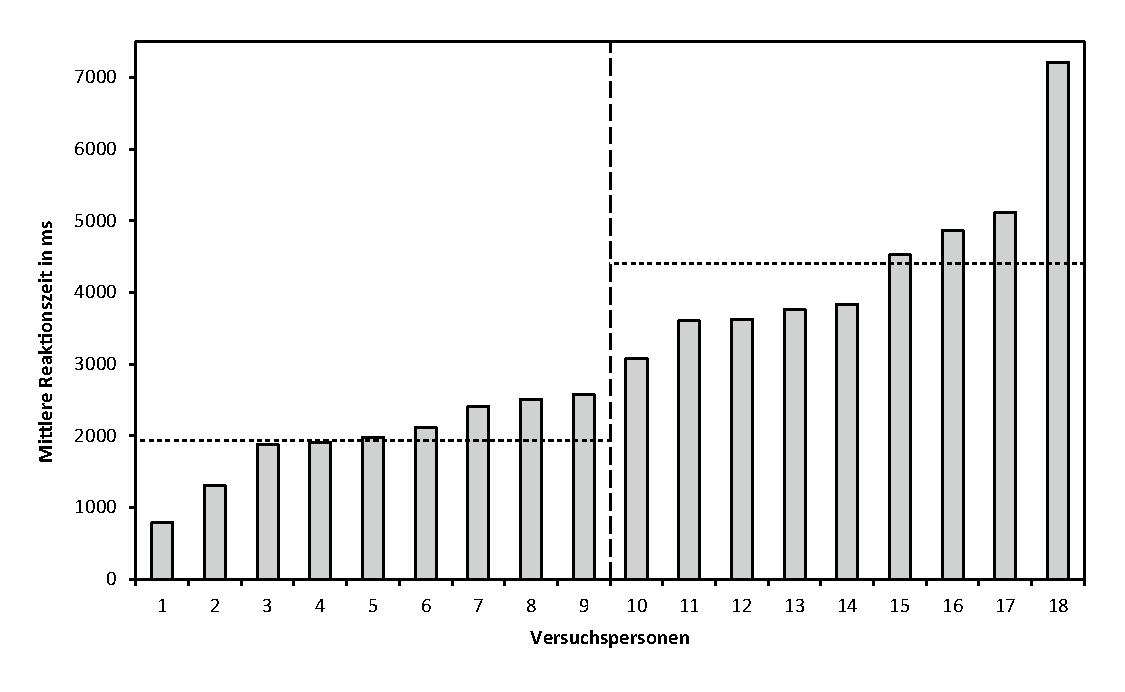
\includegraphics[width=\textwidth]{abb4-strategienV2.eps}
    \end{minipage}}
    \vspace{10pt}
    \caption[Mittelwerte der Reaktionszeiten]{Mittlere Reaktionszeit der einzelnen Versuchspersonen über alle 4 Blöcke. Die Versuchspersonen wurden mittels eines Mediansplits in zwei Gruppen getrennt. Der Trennungspunkt ist mit der gestrichelten vertikalen Linie markiert. Die gestrichelten horizontalen Linien markieren die Mittelwerte der beiden Gruppen.}
    \label{strat}
  \end{minipage}
\end{figure}

Um diese Beobachtung statistisch zu prüfen, wurden zunächst Mittelwerte der Reaktionszeiten jeder Versuchsperson über alle 4~Blöcke berechnet. Damit wurde jeder Versuchsperson eine mittlere Reaktionszeit zugeordnet. Anhand dieser Daten wurde ein Mediansplit vorgenommen. Es ergaben sich zwei Gruppen mit je 9 Versuchspersonen. Die Gruppe mit den höheren mittleren Reaktionszeiten besitzt einen Mittelwert von M~=~4400\,ms, mit einem Standardfehler von SE~=~414\,ms. Die Gruppe mit den niedrigeren mittleren Reaktionszeiten erreichte einen Mittelwert von M~=~1939\,ms und einem Standardfehler von SE~=~194\,ms. Wie anhand der Mittelwertunterschiede und in Abbildung \ref{strat} deutlich zu sehen ist, scheinen also tatsächlich zwei unterschiedliche Strategien zur Erkennung angewendet worden zu sein. Interessanterweise war jedoch keine der Gruppen besser. Bei den Versuchspersonen mit der schnellen Strategie ergab sich kein Unterschied zwischen Block~4 und Block~1 im Sensitivitätsindex, t(8)~=~1.66, p~>~0.05 und kein Unterschied zwischen Block~4 und dem Zufall, t(8)~=~-0.23, p~>~0.05. Das Gleiche ergab sich für die kognitive Strategie bei Block~4 und Block~1, t(8)~=~-0.6, p~>~0.05 und bei Block~4 gegen Zufall, t(8)~=~1.77, p~>~0.05. Auch wenn die Leistungen der Versuchspersonen innerhalb von Block~4 und zwischen den Strategien verglichen wurden, ergab sich keine signifikant bessere Leistung einer der beiden Strategien, t(15)~=~-1.54, p~>~0.05.

Es kann folglich davon ausgegangen werden, dass tatsächlich eine eher intuitive (implizite) Strategie und eine eher kognitive (explizite) Strategie angewendet wurde. Gleichzeitig führte keine von beiden Strategien zu einem besseren Ergebnis. Diese Erkenntnis stützt eher die Annahme, dass ein Lernen der komplexen Regel nicht möglich ist, da sowohl unter hohem kognitiven Aufwand, als auch bei beiläufigem  Lernen keine signifikant besseren Ergebnisse erzielt wurden.

\subsection{Effekte von Musikalität}

\begin{figure}[t]
  \centering
  \begin{minipage}{\textwidth}
    \fbox{\begin{minipage}{\textwidth}
      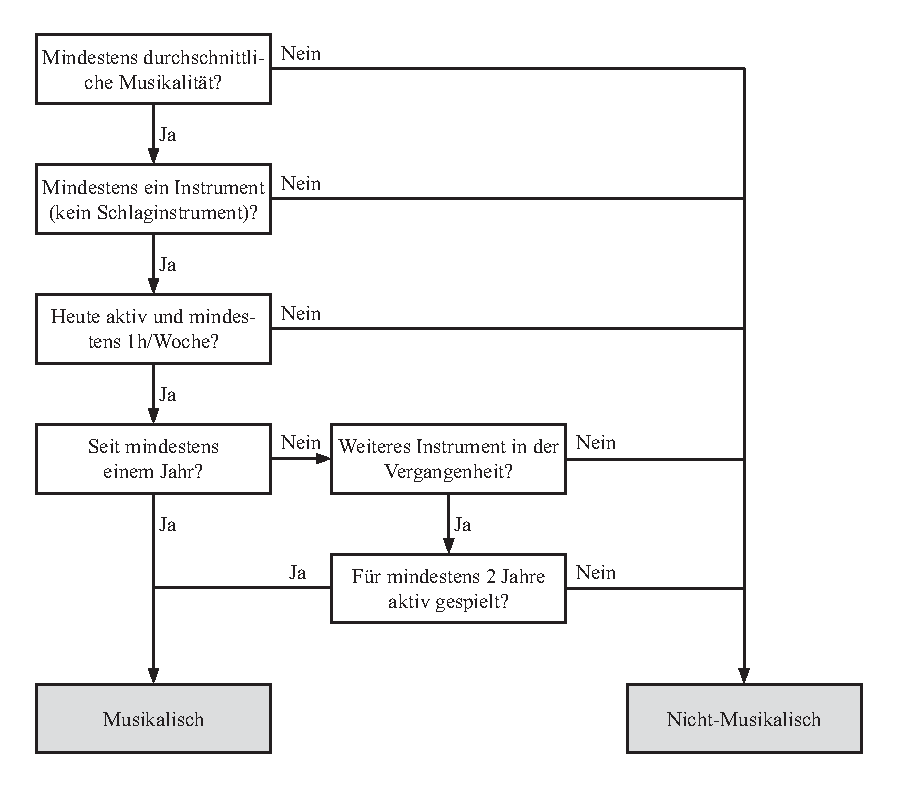
\includegraphics[width=\textwidth]{abb-musikalitaet-auswertung.eps}
    \end{minipage}}
    \vspace{10pt}
    \caption[Auswertungsschema des Fragebogens zur Musikalität]{Auswertungsschema des Fragebogens zur Musikalität (siehe Anhang) zur Kategorisierung der Versuchspersonen in musikalisch und nicht-musikalisch.}
    \label{musik:aufbau}
  \end{minipage}
\end{figure}

Nachdem Block~4 beendet war, bekamen die Versuchspersonen einen Fragebogen zur Selbsteinschätzung ihrer musikalischen Fähigkeiten (siehe Anhang). Die Versuchspersonen wurden anhand des Selbstberichtes in zwei Gruppen eingeteilt, eine musikalische und eine nicht-musikalische. Eine Versuchsperson wurde als musikalisch eingeschätzt, wenn sie zum Zeitpunkt der Erfassung angab, derzeit ein Instrument zu spielen oder zu singen, und sich selbst mindestens als durchschnittlich musikalisch einschätzt. Dabei sollte das Instrument mindestens seit einem Jahr und mindestens 1 Stunde pro Woche gespielt werden. Sollte es weniger als ein Jahr gespielt worden sein, dann muss ein zweites Instrument in der Vergangenheit für mindestens 2 Jahre gespielt worden sein. Das Schema zur Auswertung ist in Abbildung~\ref{musik:aufbau} gezeigt.

Nach dem Auswertungsschema wurden insgesamt~7 der 18~Versuchspersonen als musikalisch eingestuft (38,89\,\%). Die beiden Gruppen (musikalisch/nicht-musikalisch) unterschieden sich weder in Block~1 in ihrem Sensitivitätsindex, t(16)~=~1.27, p~>~0.05, noch in Block~4 signifikant voneinander, t(16)~=~0.51, p~>~0.05. Wie nach diesen Ergebnissen zu erwarten, ergaben sich auch innerhalb der musikalischen Personen keine Effekte. Es gab innerhalb dieser Gruppe keine Unterschiede in der Erkennungsleistung zwischen Block~1 und Block~4, t(6)~=~0.07, p~>~0.05. Auch wichen Block~1 und Block~4 nicht signifikant vom Zufall ab; t(6)~=~2.15, p~>~0.05 für Block~1 und t(6)~=~1.06, p~>~0.05 für Block~4.

Von den Ergebnissen ausgehend, haben musikalische Personen keine Vorteile durch die regelmäßige Beschäftigung mit Musik bzw. Tönen. Diese Ergebnisse sprechen dafür, dass die Informationen im Experiment tatsächlich nur sensorisch verarbeitet werden, da kein impliziter oder expliziter Lerneffekt vorliegt. Gleichzeitig sprechen die Ergebnisse dafür, dass die sensorische Verarbeitung nicht trainiert werden kann.

Einschränkend ist zu erwähnen, dass die Musikfähigkeit eher grob gemessen wurde. Interessant wären die Items des relativen und absoluten Gehörs, da diese spezifisch die Differenzierungsfähigkeit bezüglich der Tonhöhe erfasst. Diese Items konnten nicht ausgewertet werden, da zu wenige Versuchspersonen laut Selbstbericht ein gutes relatives oder ein absolutes Gehör besaßen. Mit höheren Stichproben könnten diese beiden Aspekte der Musikalität sinnvoll ausgewertet werden. Auch wäre es interessant zusätzlich einen objektiven Test einzusetzen, bei dem die Fähigkeit zur Differenzierung zwischen Tönen erfasst und die Angaben im Fragebogen überprüft werden können.

\subsection{Klassifikation}

Auf Basis der weitergehenden Analysen soll an dieser Stelle eine Begriffstrennung abgeleitet werden, die in der bisherigen Betrachtung noch nicht klar vorgenommen wurde. Die sensorische Verarbeitung kann nicht als implizit betrachtet werden, da Lerneffekte, auf deren Basis bewusste Entscheidungen getroffen werden, durch die sensorische Regelerkennung derzeit nicht nachgewiesen sind. Auch die Einordnung als prozedural oder deklarativ ist schwierig, da es keinen Bewegungsablauf gibt, es sich aber auch nicht um Wissen handelt. Letztlich ist auch der Begriff einer unbewussten Verarbeitung nicht haltbar, da eine unterbewusste Verarbeitung immer noch nachhaltige Effekte auf das Verhalten aufweist und zumindest theoretisch auch dem Bewusstsein zugänglich ist, was hier nicht der Fall ist. Die einzige Möglichkeit, den Begriff richtig einzuordnen, sehe ich im Konzept der Aufmerksamkeit. Die Einordnung als präattentiv, also vor der Aufmerksamkeit ablaufend, wie von \textcite{paavilainen2007preattentive} und \textcite{bendixen2008rapid} bereits vorgenommen, ist die einzig präzise Klassifizierung. Neu wäre an dieser Stelle, auch das implizite und explizite Lernen unter der Perspektive der Aufmerksamkeit zu betrachten.

\begin{compactitem}
  \item \textbf{Sensorisches Lernen}: Präattentive Verarbeitung (Neuronaler Lernprozess)
  \item \textbf{Implizites Lernen}: Subattentive Verarbeitung (Unbewusster Lernprozesse)
  \item \textbf{Explizites Lernen}: Attentive Verarbeitung (Bewusster Lernprozess)
\end{compactitem}

Dabei wird vorausgesetzt, dass Lernprozesse nach häufiger Übung der gleichen Einheit immer zu einer automatisierten Handlung führen. Das autonome Stadium und die Unconscious competence entspricht eben diesem automatischen Verhalten. Entscheidend ist, dass sich alle drei Mechanismen im Ergebnis ähnlich sein sollten. Der Weg zu den jeweiligen Verhaltensweisen unterscheidet sich jedoch und bildet den entscheidenden Unterschied zwischen den drei Prozessen. Hinweise dafür, dass ein Lernen auch bei impliziter und expliziter Verarbeitung möglich ist, liefern die Post-Hoc-Analysen bezüglich den - wenn auch geringen - Lernerfolgen in Block~2 und~3 und den Ergebnissen von \textcite{paavilainen2007preattentive} und \textcite{bendixen2008rapid}.

Ein weiterer Aspekt ist die Frage nach der Unabhängigkeit der Prozesse. Auf der einen Seite scheint die sensorische von der impliziten und expliziten Verarbeitung unabhängig zu sein. Obwohl auf sensorischer Ebene bereits nach wenigen Tönen eine Erkennung möglich ist, scheint dies keine Auswirkung auf die Erkennung von abweichenden Tönen zu haben. Während implizite und explizite Prozesse voneinander profitieren können \parencite{sun2005interaction}, arbeitet die sensorische Ebene wahrscheinlich isoliert. Implizite und explizite Prozesse sind außerdem weniger effektiv, jedoch adaptiv. Deutlich wurde dies daran, dass der Lernprozess auf sensorischer Ebene - angezeigt durch die MMN - bereits nach wenigen Tönen eintrat, während der Lerneffekt bei implizitem und vor allem bei explizitem Lernen nur unter sehr hohem Aufwand möglich ist. Auf der anderen Seite spricht der Ansatz der Phasenpassung des Signals mit der Oszillation des Gehirns dafür, dass eine Abhängigkeit zwischen den Prozessen besteht. Ein präattentives Signal würde nur unter bestimmten Bedingungen zu einem subattentiven oder einem attentiven Signal werden. Demnach müssten mindestens zwei Wahrnehmungsschwellen definiert werden. Eine Wahrnehmungsschwelle für die Aufnahme von Reizen in präattentive Signale und mindestens eine für den Übergang in attentive Signale, wobei auch für den Übergang von subattentiven zu attentiven Signalen eine Schwelle denkbar wäre. Das vorliegende Experiment könnte genau an der Schwelle zwischen präattentiver zu attentiver Verarbeitung liegen. Um die Unabhängigkeit der Prozesse zu prüfen, werden jedoch umfangreiche weitere Untersuchungen nötig sein.

Interessant ist außerdem, dass sich eine Einteilung der Lernprozesse aus meiner Sicht am Eindeutigsten anhand der Aufmerksamkeit vornehmen lässt. Dies ist insbesondere deshalb interessant, da es in der letzten Zeit, vor allem im Bereich der Psychotherapie, einen großes Interesse an der Erforschung des verwandten Konzeptes der Achtsamkeit (mindfulness) gibt \parencite[vgl.][]{bishop2004mindfulness,khoury2013mindfulness}. Bei der weiteren Suche nach den Zusammenhängen zwischen präattentiver, subattentiver und attentiver Verarbeitung könnte es fruchtbar sein, parallelen mit diesem Konzept im Auge zu behalten.

\subsection{Einordnung der Beispiele}

Nach der oben vorgenommenen Klassifikation lassen sich die Beispiel aus der Einleitung einordnen. In allen Beispielen ist immer eine sensorische, d.\,h. präattentive Verarbeitung vorhanden. Während bei der Fähigkeit zur Synchronisation mit Musik vermutlich zunächst primär präattentive Informationen verarbeitet werden, findet das Sprachverständnis mindestens auch auf subattentiver Ebene statt. Die Segmentation verläuft - sofern sie gut geübt ist - vermutlich eher auf subattentiver Ebene \parencite{sanders2002segmenting}, das semantische Verständnis eher auf attentiver Ebene, da kontextabhängige Informationen integriert werden können. Wörter wie `hier' oder `dort' haben je nach Ort, an dem sich eine Person befindet, eine andere Bedeutung. Der Monitoring-Prozess \parencites{levelt1983monitoring,postma2000detection} beim Sprechen erfordert wahrscheinlich eine weitgehend attentive Verarbeitung, da auch hier eine kontextabhängige Prüfung stattfinden muss. Das Gesagte muss nicht nur auf allgemeine Sprechfehler, sondern auch auf kontextuelle Passung (Zeit, Ort, etc.) überprüft werden.

\section{Zusammenfassung und Fazit}

Mit Sicherheit kann festgehalten werden, dass das Lernen einer komplexen Regel, wie sie hier angewendet wurde, sehr schwer ist, eventuell sogar unmöglich. Gleichzeitig ist festzustellen, dass das menschliche Gehirn einen Mechanismus auf sensorischer Ebene besitzt, der Regeln hocheffizient erkennen und Fehler detektieren kann. Dieser bleibt nach jetzigem Kenntnisstand einem bewussten (attentivem) Zugang verwehrt. Dabei können andere Studienergebnisse, wie die der Phasenpassung eventuell integriert werden. Folgende Studien müssten vor allem klären, ob ein explizites Lernen solcher Regeln überhaupt möglich ist. Außerdem können darauf aufbauend die Zusammenhänge zwischen präattentiver, subattentiver und attentiver Verarbeitung weiter untersucht werden.

Aber selbst nach Klärung der in der Diskussion aufgeworfenen Fragen und Ansätze bleiben die zu Beginn der Einleitung formulierten großen Fragen selbstverständlich noch unbeantwortet. Sicher aber sind weitere Untersuchungen ein Schritt in diese Richtung. Neue Hinweise werden die Möglichkeit geben weitere Theorien bilden und bestehende Theorien korrigieren zu können. Das Zusammenspiel zwischen automatischen Verhaltensweisen - als Ergebnis eines Lernprozesses - und Aufmerksamkeit - als Unterscheidungsmerkmal unterschiedlicher Lernprozesse - scheint mir eine wichtige Rolle bei dem Verständnis menschlichen Verhaltens und Erlebens einzunehmen und ein stabiler Ansatzpunkt für weitere Untersuchungen zu sein.

% ### Anhang ###
% - Fotos Versuchsaufbau
% - Arbeitsblatt
% - Musikfragebogen

\section{Literaturverzeichnis}

\printbibliography[heading=none]

\end{document}